%----------------------------------------------------------------------------------------
%	PAGE 30
%----------------------------------------------------------------------------------------
\section{Simulation}
\begin{frame}
\sectionpage
\end{frame}


%----------------------------------------------------------------------------------------
%	PAGE 31
%----------------------------------------------------------------------------------------
\begin{frame}
\frametitle{Setting}
\footnotesize
Set $n=200$, $p=3000$, and run several simulation experiments with
$100$ replications in each setting.
\begin{itemize}
\item[$\blacksquare$] Generate independent copy of $(\bX,\by)$: \\
Given a particular $\rho \in(-1,1)$, $\tilde{\bX} = (\tilde{x}_{ij})_{n\times p}$
has iid $N(0,\Sigma)$ rows with $\Sigma = (\rho^{|j-k|})_{p\times p}$,
$\bx_j = \tilde{\bx}_j\sqrt{n}/{|}\tilde{\bx}_j{|}_2$, and $(\bX,\by)$ is as in (\ref{LM}) with $\sigma=1$.
%We also set $\lam_j^*= \lambda_{univ} = \sqrt{(2/n)\log p}$.
% why do we say this here? not used in creating setup.
\item[$\blacksquare$] Generate $\bbeta$: \\
Given a particular $\alpha \geq 1$, $\beta_j = 3\lambda_{univ}$ for $j = 1500, 1800, 2100, \ldots, 3000$,
and $\beta_j = 3\lambda_{univ}/j^\alpha$ for all other $j$, where $\lambda_{univ}=\sqrt{(2/n)\log p}$.
\item[$\blacksquare$] Set $\alpha$ and $\rho$: \\
This simulation example includes four cases, labeled (A), (B), (C), and (D), respectively:
$(\alpha,\rho)=(2,\frac{1}{5})$, $(1,\frac{1}{5})$, $(2,\frac{4}{5})$, and $(1,\frac{4}{5})$.
\end{itemize}
\end{frame}


%----------------------------------------------------------------------------------------
%	PAGE 32
%----------------------------------------------------------------------------------------
\begin{frame}
\frametitle{Comparison between different methods}
\begin{figure}[h]
  \centering
  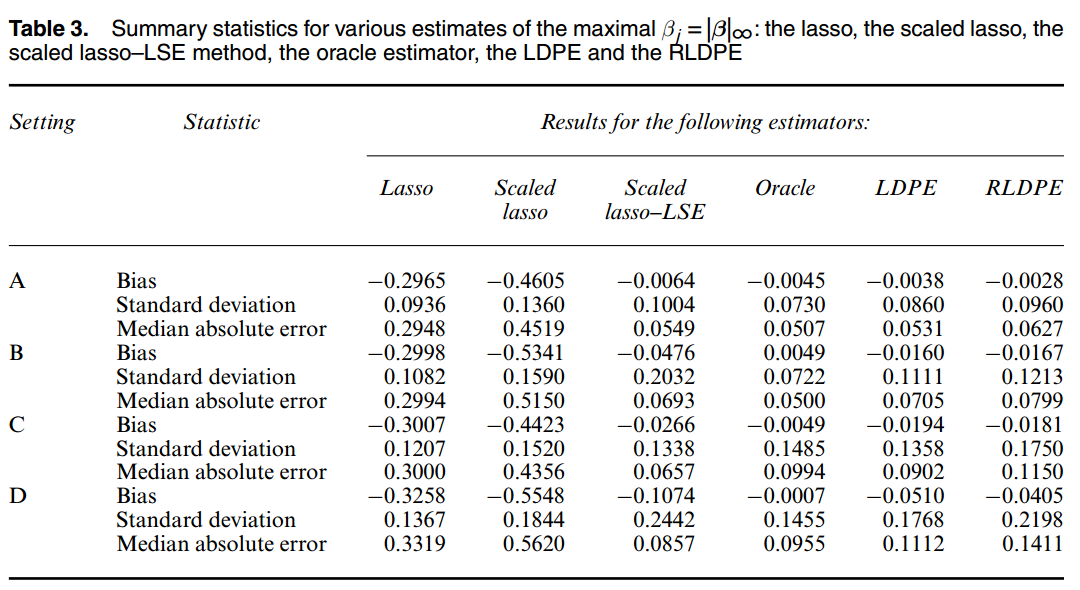
\includegraphics[width=1.0\textwidth]{figs/Table3.png}
  \label{Table1}
\end{figure}
\end{frame}


%----------------------------------------------------------------------------------------
%	PAGE 33
%----------------------------------------------------------------------------------------
\begin{frame}
\frametitle{Histogram of error}
%\begin{figure}[h]
%  \centering
%  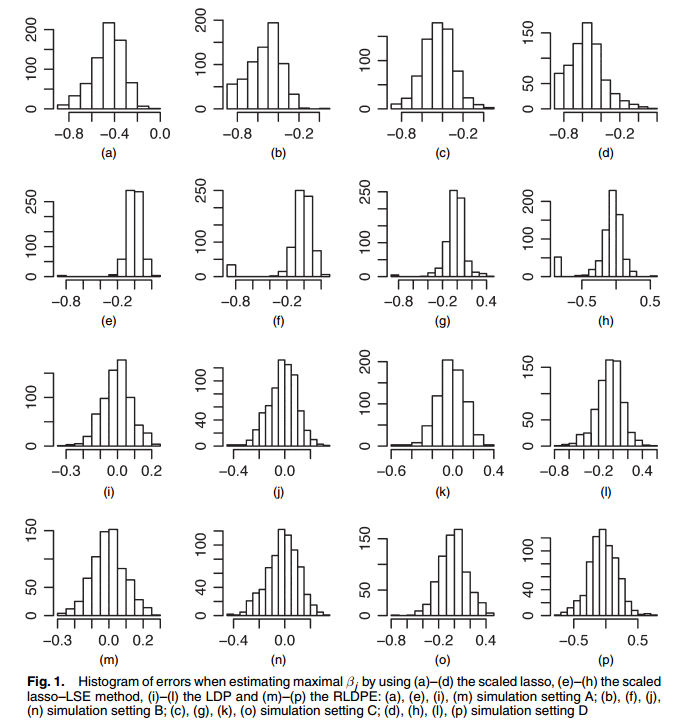
\includegraphics[width=1\textwidth]{figs/Table 4.png}
%  \label{Table4}
%\end{figure}
%\end{frame}

\begin{centering}
\begin{figure}[t]
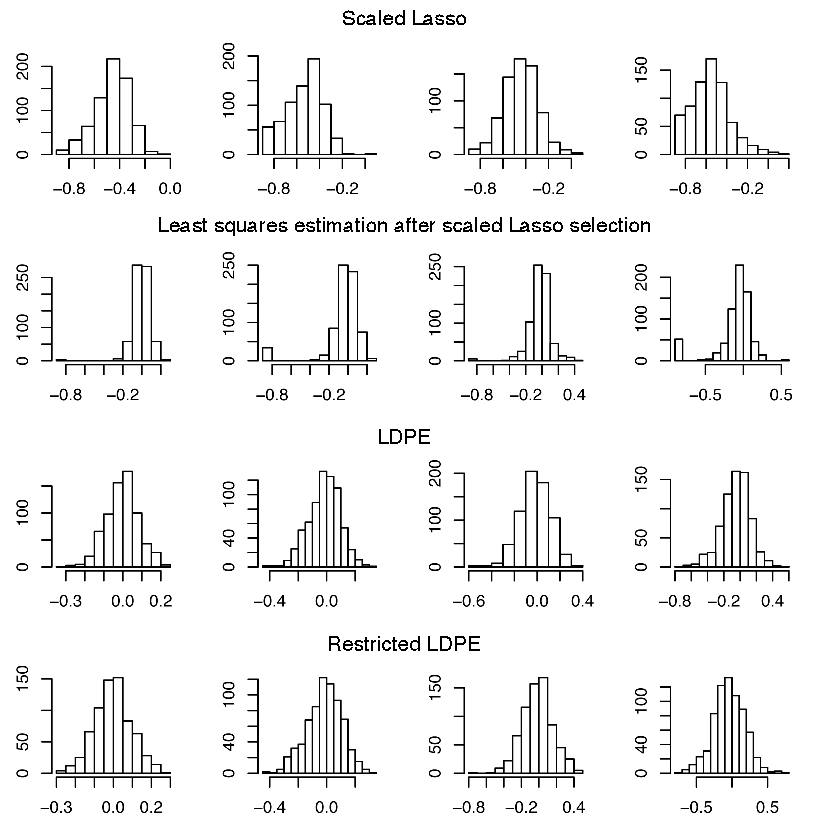
\includegraphics[width = 0.65\textwidth]{1110/hist_diff.pdf}
%\caption{Histogram of errors when estimating maximal $\beta_j$ using the scaled Lasso,
%{the scaled Lasso-LSE}, the LDPE, and the {R-LDPE}. From left to right,
%plots correspond to simulation settings (A), (B), (C), and (D).}
\label{fig:hist}
\end{figure}
\end{centering}

\end{frame}


%----------------------------------------------------------------------------------------
%	PAGE 34
%----------------------------------------------------------------------------------------
\begin{frame}
\frametitle{Result of mean coverage probability}

\begin{table}[ht]
\caption{Mean coverage probability of LDPE and R-LDPE.}
\begin{tabular}{llcccc}
\toprule
&&A&B&C&D\\
\midrule
all $\beta_j$& LDPE & $0.9597$ & $0.9845$ & $0.9556$ & $0.9855$ \\
 &R-LDPE & $0.9595$ & $0.9848$ & $0.9557$ & $0.9885$  \\ [1ex]
 maximal $\beta_j$ & LDPE&  $0.9571$ & $0.9814$& $0.9029$ &$0.9443$\\
& R-LDPE & $0.9614$ & $0.9786$ & $0.9414$ & $0.9786$\\
\bottomrule
\end{tabular}

\label{table:meancover}
\end{table}
\end{frame}


%----------------------------------------------------------------------------------------
%	PAGE 35
%----------------------------------------------------------------------------------------
\begin{frame}
\begin{centering}
\begin{figure}[p]
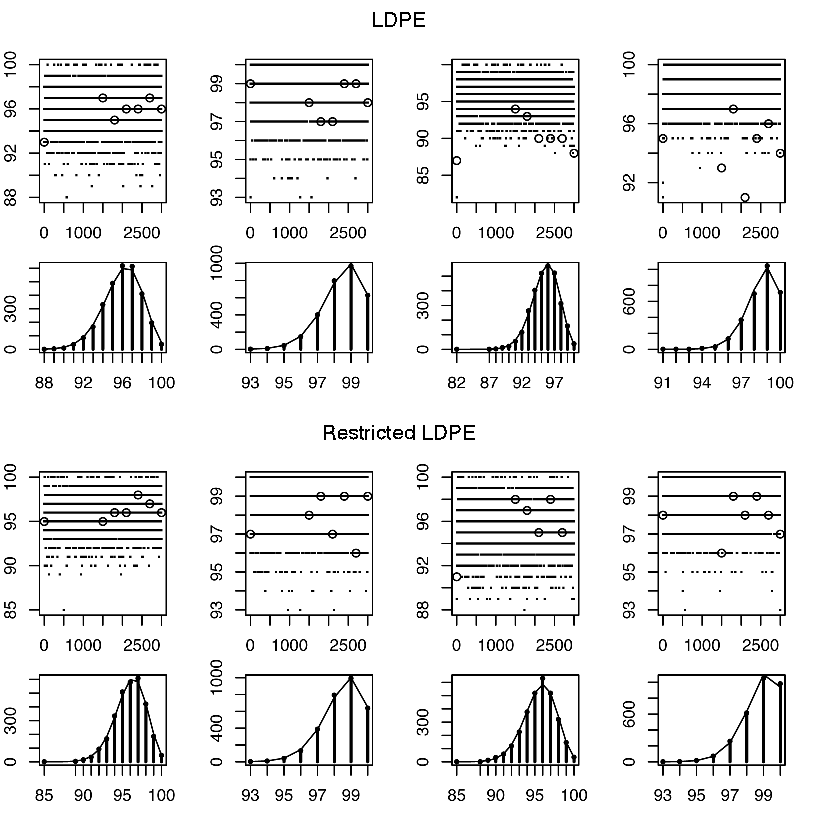
\includegraphics[width = 8cm]{1110/coverage.pdf}
%\caption{Rows 1 and 3: Coverage frequencies versus the index of $\beta_j$. Points corresponding to maximal $\beta_j$ are plotted as large circles. Rows 2 and 4: The number %percentage of variables for given values of the relative coverage frequency, superimposed n the binomial$(100,\tilde p)$ probability mass function, where $\tilde p$ is the simulated mean coverage. Figures depict results from simulations A, B, C, and D, from left to right.}
\label{fig:cover}
\end{figure}
\end{centering}

\end{frame}

%----------------------------------------------------------------------------------------
%	PAGE  刘磊的实验结果_1
%----------------------------------------------------------------------------------------
\begin{frame}
\frametitle{Simulation 1: Summary statistics for different estimators}
We set $p=300, n=50$, replication$=100$, let $\Sigma, \alpha=2, \rho=1/5$ the same as Setting A. %Generating design matrix $\bX$ from different $\Sigma$ to compare the mean coverage probability by LDPE.

\begin{table}[ht]
\caption{Summary statistics for different estimators of the maximal $\beta_j = \| \beta \|_{\infty}$}
\begin{tabular}{lcccc}
\toprule
&Lasso&Scaled lasso&LDPE \\
\midrule
Bias & $2.070$ & $2.110$ & $0.580$ \\
Standard deviation & $0.046$ & $0.042$ & $0.181$ \\
\bottomrule
\end{tabular}
\label{liu1}

\end{table}
\end{frame}

%\begin{table}
%\centering
%\caption{Mean Coverage}
%\begin{tabular}{cccc}
%\toprule
%Setting             &   Method       & All   & Maximal\\
%\midrule
%\multirow{2}*{ A }  &   $\ell_{0}$   & 0.915 & 0.930 \\
%                    &   Scaled lasso & 0.907 & 0.920 \\
%\multirow{2}*{ B }  &   $\ell_{0}$   & 0.942 & 0.980 \\
%                        Scaled lasso & 0.953 & 0.970 \\
%\bottomrule
%\end{tabular}
%\end{table}

%----------------------------------------------------------------------------------------
%	PAGE  刘磊的实验结果_2
%----------------------------------------------------------------------------------------
\begin{frame}
\frametitle{Simulation 2: Mean coverage probability}
We set $p=300, n=50$, replication$=100$. Generating design matrix $\bX$ from different $\Sigma$ to compare the mean coverage probability by LDPE.
\begin{itemize}
\item[$\blacktriangleright$] Setting A: $\Sigma=(\rho^{|j-k|})_{p\times p}, \rho = 0.2$
\item[$\blacktriangleright$] Setting B: $\Sigma=(\rho^{|j-k|})_{p\times p}, \rho = 0.8$
\item[$\blacktriangleright$] Setting C: $\Sigma=(\rho)_{p\times p}, j\neq k, \rho = 0.2$
\item[$\blacktriangleright$] Setting D: $\Sigma=(\rho)_{p\times p}, j\neq k, \rho = 0.8$
\end{itemize}

\begin{table}[h]
\caption{Mean coverage probability of LDPE.}
\begin{tabular}{lcccc}
\toprule
&A&B&C&D\\
\midrule
all $\beta_j$& $0.919$ & $0.934$ & $0.910$ & $0.913$ \\
maximal $\beta_j$& $0.940$ & $0.980$ & $0.950$ & $0.960$ \\
\bottomrule
\end{tabular}

\label{liu2}
\end{table}
\end{frame}


%----------------------------------------------------------------------------------------
%	PAGE  刘磊的实验结果_3
%----------------------------------------------------------------------------------------
\begin{frame}
\frametitle{Simulation 3: Choosing initial estimator of $\bbeta$ by $\ell_0$ and scaled lasso}
We set $p=300$, $n=50$, replication=100. $\beta_{j}=3\lambda_{univ}$ for $j=15,18,\ldots,30$, and $\beta_{j}=3\lambda_{univ}/j^{\alpha}$ for other $j$.
\begin{itemize}
\item[$\blacktriangleright$] Setting A: $\Sigma=(\rho^{|j-k|})_{p\times p}, \rho = 0.2$
\item[$\blacktriangleright$] Setting B: $\Sigma=(\rho^{|j-k|})_{p\times p}, \rho = 0.6$
\end{itemize}
\begin{table}[ht]
\caption{Mean coverage probability of $\ell_{0}$ and Scaled lasso.}
\begin{tabular}{llcc}
\toprule
&&A&B\\
\midrule
all $\beta_j$ &$\ell_{0}$ & $0.915$ & $0.942$ \\
&Scaled lasso & $0.907$ & $0.953$ \\[1ex]
maximal $\beta_j$ &$\ell_{0}$ & $0.930$ & $0.980$ \\
&Scaled lasso & $0.920$ & $0.970$ \\
\bottomrule
\end{tabular}

\label{liu3}
\end{table}
\end{frame}
